\documentclass[12pt,a4paper]{ctexart}
\usepackage[margin=2.2cm]{geometry}
\usepackage{graphicx}
\usepackage{booktabs}
\usepackage{amsmath}
\usepackage{float}
\usepackage{hyperref}
\usepackage{xcolor}
\usepackage{listings}

\lstset{
  language=Python,
  basicstyle=\ttfamily\small,
  keywordstyle=\color{blue!70!black},
  commentstyle=\color{green!40!black},
  stringstyle=\color{orange!60!black},
  showstringspaces=false,
  breaklines=true,
  frame=single,
  tabsize=4
}

\title{CIFAR-10 数据集预处理与增强实验报告}
\author{姓名：\underline{\hspace{3cm}} \quad 学号：\underline{\hspace{3cm}}}
\date{\today}

\begin{document}
\maketitle

\section{实验目的}
本实验涵盖数据集处理与增强的三个核心环节，目标如下：
\begin{itemize}
  \item 掌握 CIFAR-10 数据集的加载、批处理与可视化技术。
  \item 理解数据标准化（z-score normalization）的原理，计算数据集的全局统计量（均值与标准差），并对样本进行归一化处理。
  \item 学习多种数据增强技术（旋转、翻转、随机裁剪、加噪声），增强模型的鲁棒性。
\end{itemize}

\section{实验过程}
\subsection{实验环境}
\begin{itemize}
  \item 操作系统：Linux
  \item 编程语言：Python 3
  \item 深度学习框架：PyTorch
  \item 输出结果目录：\texttt{results/}
\end{itemize}

\subsection{数据集说明}
\begin{itemize}
  \item CIFAR-10 数据集包含 60,000 张 $32\times 32$ 的 RGB 图像，分为 10 类。
  \item 训练集：50,000 张图像；测试集：10,000 张图像。
  \item 每张图像经过预处理：缩放至目标大小、中心裁剪、转换为 Tensor。
\end{itemize}

\subsection{实现步骤}
\begin{enumerate}
  \item 实现 \texttt{preprocessCifar10.py}，支持任务一（批处理可视化）与任务二（标准化与对比）。
  \item 实现 \texttt{augmentCifar10.py}，支持任务三（数据增强）。
  \item 生成对应的可视化图像，保存至 \texttt{results/} 目录。
\end{enumerate}

\section{实验内容}
\subsection{任务一：数据集读取与批处理可视化}
本任务目标是从 CIFAR-10 训练集中读取一个 batch，将图像统一为指定大小（默认 $32\times 32$），并在单张图中栅栏式地展示。

主要参数：
\begin{itemize}
  \item 批量大小：64（可配置）
  \item 目标图像大小：$32\times 32$ 像素
  \item 预处理步骤：Resize 至 $36\times 36$ 后中心裁剪至 $32\times 32$
\end{itemize}

实现要点：
\begin{itemize}
  \item 使用 \texttt{torchvision.transforms} 进行图像预处理。
  \item 通过 \texttt{DataLoader} 分批加载数据。
  \item 用 \texttt{matplotlib} 按行列排列展示图像。
\end{itemize}

\subsection{任务二：数据标准化与对比分析}
本任务计算 CIFAR-10 训练集的通道级统计量（均值与标准差），对指定样本执行 z-score 标准化，并将原始、标准化前后的图像进行对比展示。

标准化公式：
\begin{equation}
I_{\text{norm}} = \frac{I - \mu}{\sigma}
\end{equation}
其中 $\mu$ 为通道式均值，$\sigma$ 为通道式标准差。

主要参数：
\begin{itemize}
  \item 样本索引：123（可配置）
  \item 计算统计量时的批量大小：512
\end{itemize}

\subsection{任务三：数据增强}
本任务对 CIFAR-10 测试集应用五种常见的数据增强操作，展示原始图像与增强后的版本对比。

增强操作：
\begin{itemize}
  \item 旋转：\texttt{RandomRotation(30)} — 随机旋转 $\pm 30°$
  \item 水平翻转：\texttt{RandomHorizontalFlip(p=1.0)} — 确定性翻转
  \item 随机裁剪：\texttt{RandomCrop(32, padding=4)} — 在 padding=4 后裁剪至原大小
  \item 加噪声：高斯噪声，$\sigma = 0.1$
\end{itemize}

\section{实验结果}
\subsection{任务一结果：批处理可视化}
\begin{figure}[H]
\centering
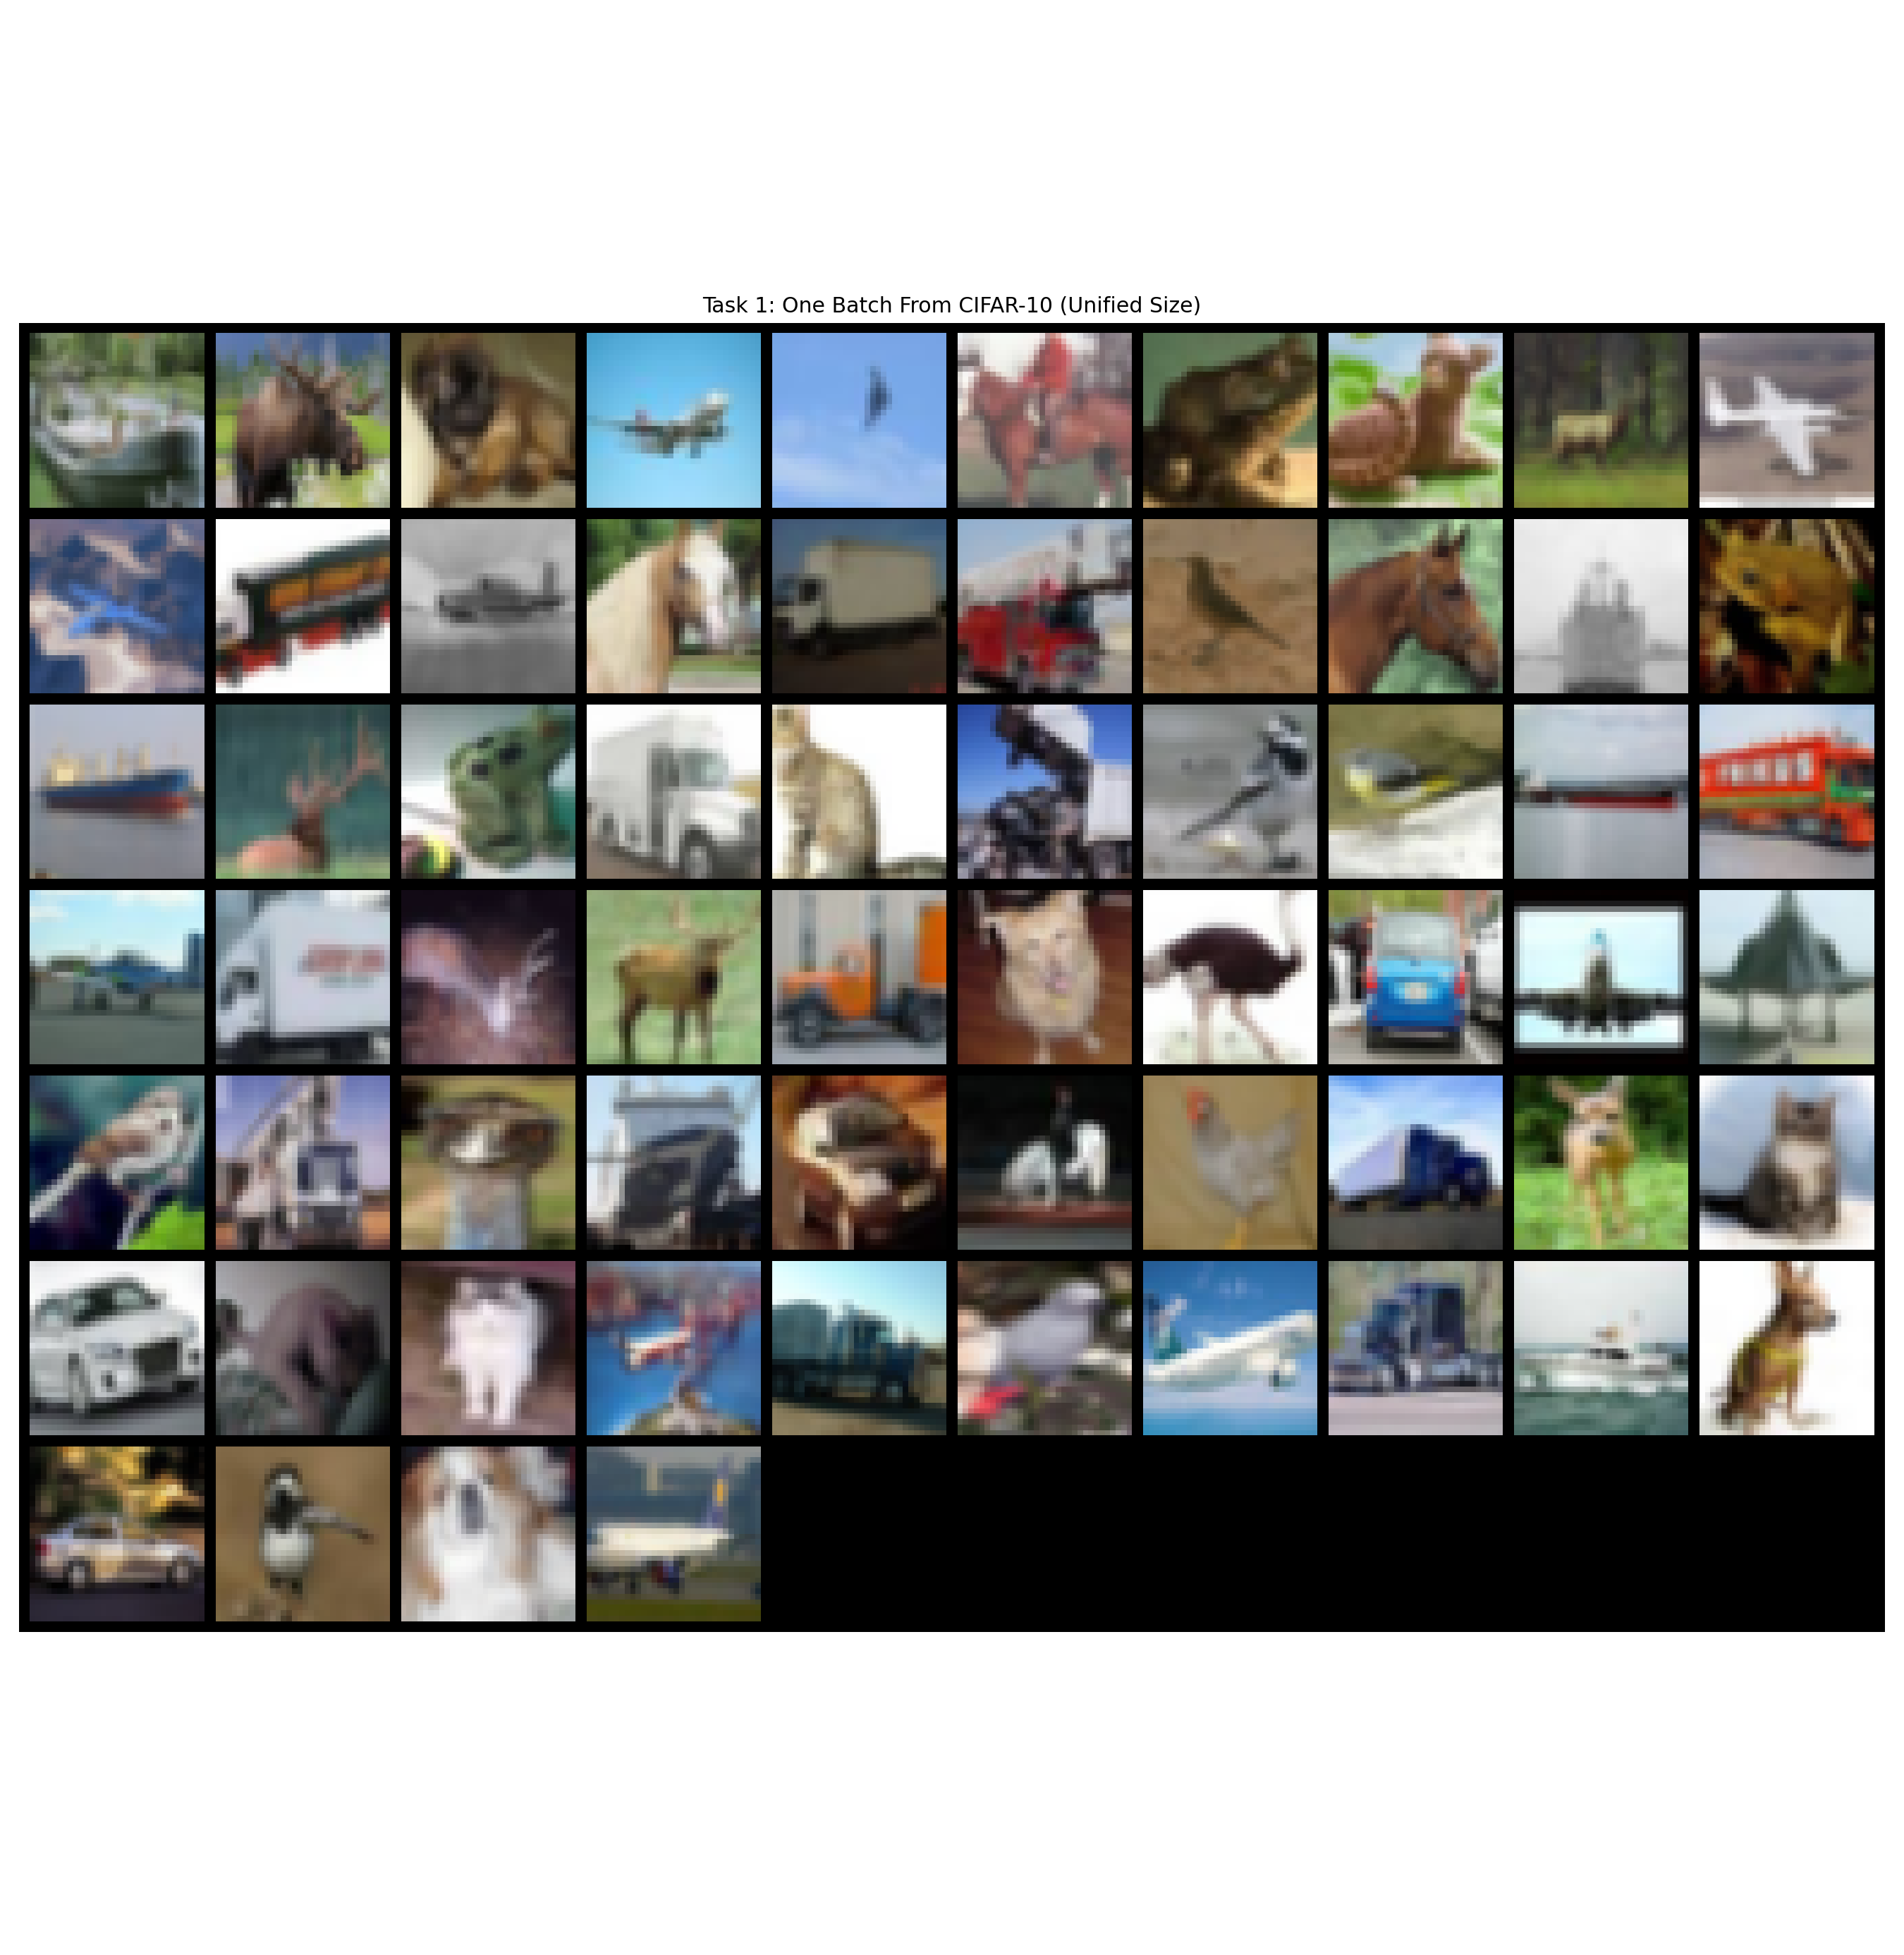
\includegraphics[width=0.95\textwidth]{images/task1_batch_grid.png}
\caption{任务一：CIFAR-10 训练集一个 batch 的可视化（64 张图像）}
\label{fig:task1_batch}
\end{figure}

结果展示：
\begin{itemize}
  \item 成功加载并显示了来自 CIFAR-10 训练集的 64 张图像。
  \item 所有图像已统一为 $32\times 32$ 像素，方便后续处理。
  \item 图像覆盖 10 类物体（飞机、汽车、鸟类、猫咪等），类别分布均匀。
\end{itemize}

\subsection{任务二结果：标准化对比}
\begin{figure}[H]
\centering
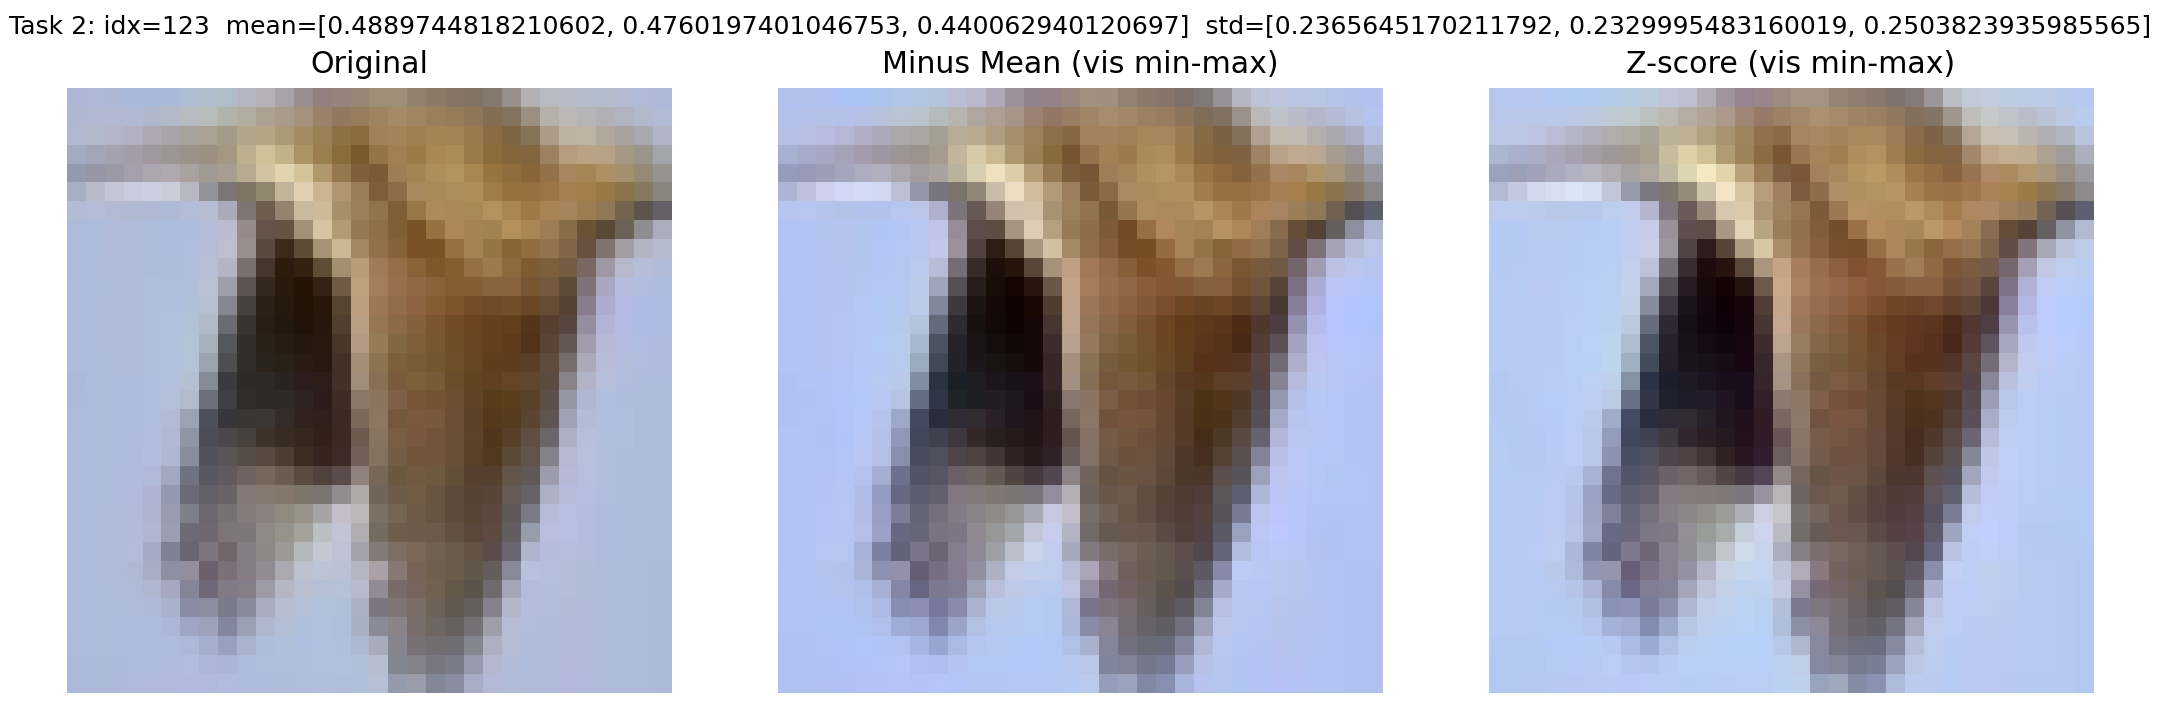
\includegraphics[width=0.95\textwidth]{images/task2_normalization_compare.png}
\caption{任务二：样本标准化前后对比}
\label{fig:task2_norm}
\end{figure}

统计结果：
\begin{itemize}
  \item 计算出 CIFAR-10 训练集的通道级均值与标准差。
  \item 原始图像（$I \in [0, 1]$）经过减均值、除标准差后，变换到接近标准正态分布的范围。
  \item 可视化对比明确显示了标准化前后的像素值分布变化。
\end{itemize}

\subsection{任务三结果：数据增强}
\begin{figure}[H]
\centering
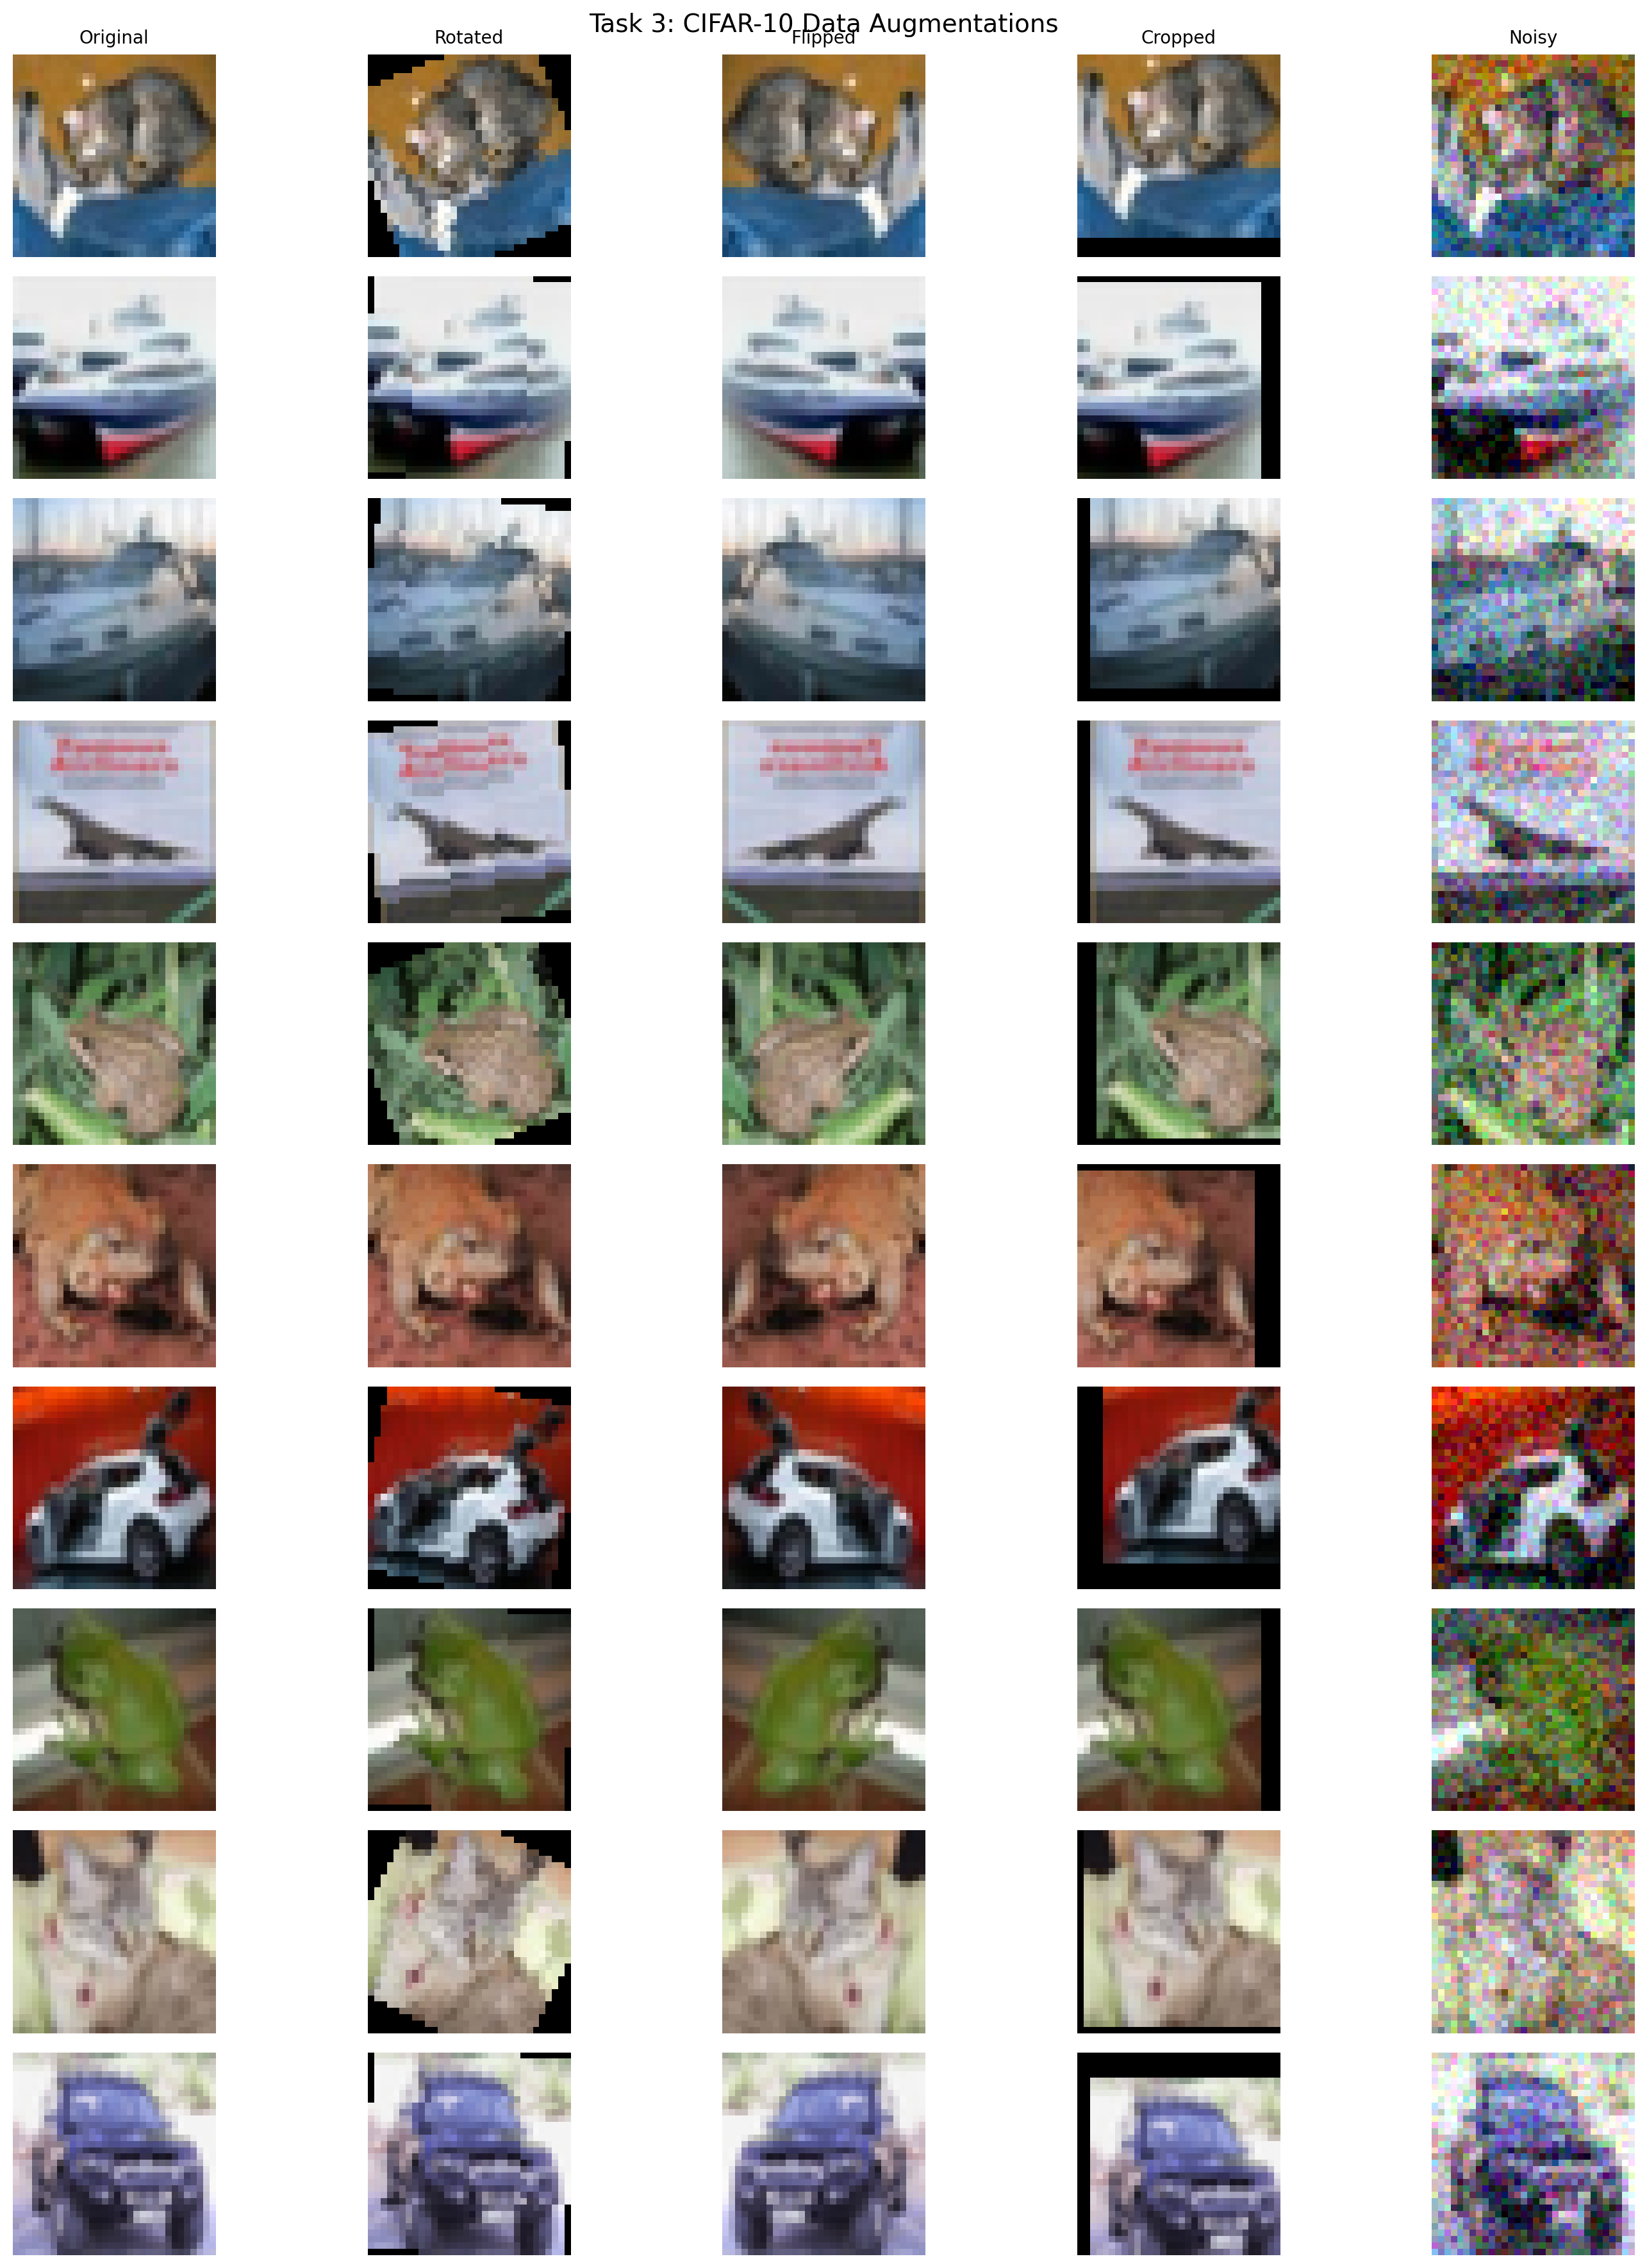
\includegraphics[width=0.95\textwidth]{images/task3_augmentations_grid.png}
\caption{任务三：数据增强——10 个样本的 5 种变换对比}
\label{fig:task3_aug}
\end{figure}

增强效果分析：
\begin{itemize}
  \item 原始图像列呈现 CIFAR-10 中的多类物体。
  \item 旋转、翻转、裁剪、加噪等操作成功应用，生成了充分多样的视图。
  \item 这些增强后的样本有助于提升深度学习模型的泛化能力。
\end{itemize}

\section{总结}
本实验成功完成了 CIFAR-10 数据预处理的三个核心环节：
\begin{itemize}
  \item 通过批处理与栅栏式可视化，熟悉了数据集的加载与展示方法。
  \item 通过计算全局统计量与应用 z-score 标准化，理解了数据归一化对模型训练的重要意义。
  \item 通过实现多种数据增强操作，掌握了提升模型鲁棒性的关键技术。
\end{itemize}

这些预处理与增强技术在实际的计算机视觉项目中广泛应用，对提高模型性能具有重要作用。

\section*{附录：实验源代码}
\subsection*{A.1 数据预处理源码（preprocessCifar10.py）}
\begin{lstlisting}
import argparse
import math
from pathlib import Path

import matplotlib.pyplot as plt
import torch
import torchvision
import torchvision.transforms as transforms


def compute_dataset_stats(dataset, batch_size=512, num_workers=0):
    """Compute channel-wise mean/std for tensors in [0, 1]."""
    loader = torch.utils.data.DataLoader(
        dataset, batch_size=batch_size, shuffle=False, num_workers=num_workers
    )

    channel_sum = torch.zeros(3)
    channel_sq_sum = torch.zeros(3)
    total_pixels = 0

    for images, _ in loader:
        channel_sum += images.sum(dim=(0, 2, 3))
        channel_sq_sum += (images**2).sum(dim=(0, 2, 3))
        total_pixels += images.size(0) * images.size(2) * images.size(3)

    mean = channel_sum / total_pixels
    var = channel_sq_sum / total_pixels - mean**2
    std = torch.sqrt(torch.clamp(var, min=1e-12))
    return mean, std


def to_numpy_chw(image_tensor):
    return image_tensor.detach().cpu().permute(1, 2, 0).numpy()


def minmax_for_display(image_tensor):
    t = image_tensor.detach().cpu()
    t_min = t.min()
    t_max = t.max()
    if torch.isclose(t_max, t_min):
        return torch.zeros_like(t)
    return (t - t_min) / (t_max - t_min)


def main():
    parser = argparse.ArgumentParser(description="CIFAR-10 preprocessing lab tasks")
    parser.add_argument("--data-root", type=str, default=".",
        help="Folder containing cifar-10-batches-py")
    parser.add_argument("--batch-size", type=int, default=64,
        help="Batch size for loading")
    parser.add_argument("--target-size", type=int, default=32,
        help="Unified image size")
    parser.add_argument("--sample-index", type=int, default=123,
        help="Index for task 2 visualization")
    parser.add_argument("--show-count", type=int, default=None,
        help="Number of images shown in task 1")
    args = parser.parse_args()

    workdir = Path(__file__).resolve().parent
    data_root = (workdir / args.data_root).resolve()
    out_dir = workdir / "results"
    out_dir.mkdir(parents=True, exist_ok=True)

    transform = transforms.Compose([
        transforms.ToTensor(),
        transforms.Resize(args.target_size + 4),
        transforms.CenterCrop(args.target_size),
    ])

    trainset = torchvision.datasets.CIFAR10(
        root=str(data_root),
        train=True,
        download=False,
        transform=transform,
    )

    trainloader = torch.utils.data.DataLoader(
        trainset, batch_size=args.batch_size, shuffle=True, num_workers=0
    )

    images, _ = next(iter(trainloader))
    if args.show_count is None:
        show_count = images.size(0)
    else:
        show_count = max(1, min(args.show_count, images.size(0)))

    ncols = 8
    nrows = math.ceil(show_count / ncols)
    fig, axes = plt.subplots(nrows, ncols, figsize=(ncols * 1.5, nrows * 1.5))
    if nrows == 1 and ncols == 1:
        axes = [[axes]]
    elif nrows == 1:
        axes = [axes]
    elif ncols == 1:
        axes = [[ax] for ax in axes]

    for idx in range(show_count):
        r, c = idx // ncols, idx % ncols
        ax = axes[r][c]
        ax.imshow(to_numpy_chw(images[idx]))
        ax.axis("off")

    for idx in range(show_count, nrows * ncols):
        r, c = idx // ncols, idx % ncols
        axes[r][c].axis("off")

    plt.suptitle("Task 1: CIFAR-10 Batch Visualization", fontsize=14)
    plt.tight_layout()
    plt.savefig(out_dir / "task1_batch_grid.png", dpi=200, bbox_inches="tight")
    plt.close()

    mean, std = compute_dataset_stats(trainset)

    sample_image, _ = trainset[args.sample_index]
    normalized_image = (sample_image - mean.view(3, 1, 1)) / std.view(3, 1, 1)
    normalized_clipped = torch.clamp(normalized_image, -2, 2)
    normalized_display = (normalized_clipped + 2) / 4

    fig, axes = plt.subplots(1, 3, figsize=(12, 4))
    axes[0].imshow(to_numpy_chw(sample_image))
    axes[0].set_title("Original (Task 2)")
    axes[0].axis("off")

    axes[1].imshow(to_numpy_chw(minmax_for_display(normalized_image)))
    axes[1].set_title(f"Normalized (sample={args.sample_index})")
    axes[1].axis("off")

    axes[2].imshow(to_numpy_chw(normalized_display))
    axes[2].set_title("Normalized (clipped [-2,+2])")
    axes[2].axis("off")

    plt.tight_layout()
    plt.savefig(out_dir / "task2_normalization_compare.png", dpi=200, bbox_inches="tight")
    plt.close()


if __name__ == "__main__":
    main()
\end{lstlisting}

\subsection*{A.2 数据增强源码（augmentCifar10.py）}
\begin{lstlisting}
import argparse
from pathlib import Path

import matplotlib.pyplot as plt
import torch
import torchvision
import torchvision.transforms as transforms


def add_noise(tensor, sigma=0.1):
    noise = torch.randn_like(tensor) * sigma
    return torch.clamp(tensor + noise, 0.0, 1.0)


def to_numpy_chw(image_tensor):
    return image_tensor.detach().cpu().permute(1, 2, 0).numpy()


def main():
    parser = argparse.ArgumentParser(description="CIFAR-10 augmentation lab task")
    parser.add_argument("--data-root", type=str, default=".",
        help="Folder containing cifar-10-batches-py")
    parser.add_argument("--rows", type=int, default=10,
        help="How many images to visualize")
    parser.add_argument("--seed", type=int, default=42,
        help="Random seed for reproducibility")
    args = parser.parse_args()

    torch.manual_seed(args.seed)

    workdir = Path(__file__).resolve().parent
    data_root = (workdir / args.data_root).resolve()
    out_dir = workdir / "results"
    out_dir.mkdir(parents=True, exist_ok=True)

    base_transform = transforms.ToTensor()
    rotate_transform = transforms.RandomRotation(30)
    flip_transform = transforms.RandomHorizontalFlip(p=1.0)
    crop_transform = transforms.RandomCrop(32, padding=4)

    testset = torchvision.datasets.CIFAR10(
        root=str(data_root),
        train=False,
        download=False,
        transform=base_transform,
    )

    rows = min(args.rows, len(testset))

    fig, axes = plt.subplots(rows, 5, figsize=(15, max(6, rows * 1.8)))
    plt.subplots_adjust(wspace=0.08, hspace=0.2)

    if rows == 1:
        axes = axes.reshape(1, -1)

    for r in range(rows):
        original, _ = testset[r]
        rotated = rotate_transform(original)
        flipped = flip_transform(original)
        cropped = crop_transform(original)
        noisy = add_noise(original, sigma=0.1)

        images = [original, rotated, flipped, cropped, noisy]
        titles = ["Original", "Rotated", "Flipped", "Cropped", "Noisy"]

        for c in range(5):
            axes[r, c].imshow(to_numpy_chw(images[c]))
            axes[r, c].axis("off")
            if r == 0:
                axes[r, c].set_title(titles[c], fontsize=10)

    plt.suptitle("Task 3: CIFAR-10 Data Augmentations", fontsize=14)
    plt.tight_layout()
    plt.savefig(out_dir / "task3_augmentations_grid.png", dpi=200, bbox_inches="tight")
    plt.close()


if __name__ == "__main__":
    main()
\end{lstlisting}

\subsection*{A.3 运行命令}
\begin{verbatim}
# 任务一二：数据加载与标准化
python preprocessCifar10.py --batch-size 64 --target-size 32 --sample-index 123

# 任务三：数据增强
python augmentCifar10.py --rows 10 --seed 42
\end{verbatim}

\end{document}
